\documentclass{article}
\usepackage[utf8]{inputenc}
\usepackage{verbatim}
\usepackage{graphicx}
\graphicspath{ {./images/} }


\title{\Huge Machine Learning Retrieval Report: SVM Ranking\\}
\author{\Large Beatrice Olivari, Cristian Abrante Dorta,\\
\Large Junhui Liang, Yanyun Wang}
\date{March 2020}

\begin{document}

\maketitle

\section{Introduction}
In this paper we are going to describe a method used in Machine Learning Retrieval (MLR). The aim is to rank a list of documents that appear in a query, according to their relevance. In particular, we have been given three queries in the medical field. Each query is composed by the tokens of the query and the list of papers ranked as they should be in the search engine. The task consists in building a training set with these data and implement an algorithm which will be trained with this set and will give us a new rank based on the method used.

\section{The SVM method for ranking}
Among the three possible Machine Learning Retrieval methods seen in class, we have chosen to present the SVM-Rank, a pairwise method based on clickthrough data.
This algorithm was published by Thorsten Joachims in 2002.
First of all, as already mentioned, SVM is a pairwise method. This means that it is based on a binary relation with compares two documents saying which of them should be ranked higher than the other. 
Moreover, it is based on clickthrough data. This means that for each query we do not have an expert saying which of the results are the most relevant, but we base the relevance judgment on what users click. This peculiarity also involves another characteristic of SVM, which is the fact that it does not convey absolute relevance. Since users typically scan only the first n links of the ranking, clicking on a link cannot be interpreted as a relevance judgment on an absolute scale. Maybe a document ranked much lower in the list was much more relevant, but the user never saw it.

\section{How to train our model}

\subsection{Storing clickthrough data for the training process}
The first step of the training process (and also a very important one) is to decide how to store data. First of all, it should be mentioned that the data we are looking for are extremely easy to get: in contrast to users feedback data, clickthough are simply hidden in the logfiles. Using these data is also highly practical due to the fact that they are free, available in high quantities and time convenient.\\
That being said, how do we store this big amount of data in order to make them functional for the algorithm?
As suggested by Professor Thorsten Joachims, we decided to store each query as a triplet (q,r,c). Let's describe these three components using the "Blood glucose" query as an example.
\begin{itemize}
\item q is the query, identified by both a query ID and a string with the tokens. In the example case, the ID is 0 and the tokens are the two words composing "Blood Glucose"
\item r is the ranking of the documents presented to the users (identified by an ID) and in our query it is represented by the ranked list of all the documents.
\item c is the list of links the user clicked on, which in our example is a list of 6 documents.
\end{itemize}

\subsection{The learning process}

We already mentioned in the previous section that SVM does not give us an absolute relevant judgment. With reference to the figure \ref{fig:bloodglucose}, for example, we can see that the document five was the first one the user clicked on. By noticing this, we can state that document 5 is more relevant for the user than the previous four documents. Why can we assert this? Because it is logical to think that scanning the results, the user will follow the ranking from the top to the bottom.
Nevertheless, we cannot state that, for example, document 20 is not relevant at all, just because the user did not click on it. We also have to consider that perhaps the user did not go through all the list, but stopped before.\\

\begin{figure}[h]
    \centering
    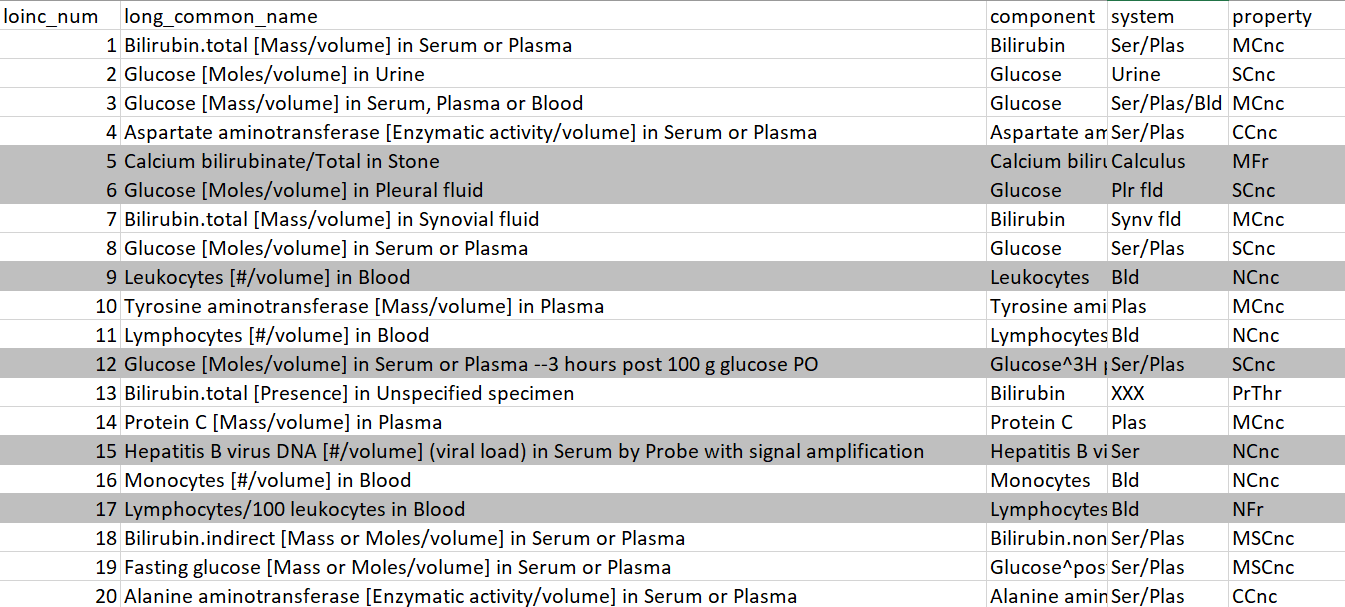
\includegraphics[scale=0.3]{Blood glucose query.png}
    \caption{"Blood glucose" query: the rows coloured in gray correspond to the ones the user clicked on.}
    \label{fig:bloodglucose}
\end{figure}

The order of the documents in the page of the query is only one of the features that the algorithm should take in account during the learning process. Another feature which is used frequently is the number of words shared by the document and the query tokens. Other examples are: BM25, document length of the body or of the title, etc.\\

The aim of the algorithm is to find a system that gives us an optimal ranking r*, however it is almost impossible to reach the optimum order, therefore what we are looking for is a function f that sorts the document with an order r\textsubscript{f(q)} which must be as similar as possible to the optimal one.\\

As we know, for a learning algorithm to be performed and to improve we have to give him some sort of evaluation. In this case we can use the statistical Kendall's tau, which was invented to find the correlation between two random variables. In our case the two variables are the actual ranking r\textsubscript{f} and the optimal ranking r*. The formula is:
\[\tau( r*,  r\textsubscript{f(q)}) = \frac{P-Q}{P+Q}\]
Being P the number of concordant pairs and Q the number of discordant ones.\\

The Kendall's tau calculates the distance of the ranking made by f on a specific query q and the optimal ranking for that query r*. In general what we want to find with the learning process is the function f that maximizes the following integral sum.
\[\tau\textsubscript{P}(f) = \int_{}{} \tau(r\textsubscript{f(q)},r*)dPr(q,r*)\]

Even though theoretically the formula presented above is the one that has to be optimize, in practice, most of the MLR method do not actually use it, but a simplified formulation.
Given a training sample S of size n (in our case the size is three cause the sample is composed by our three queries) containing queries with their target rankings r*
\[(q\textsubscript{1}, r\textsubscript{1}*), (q\textsubscript{2}, r\textsubscript{2}*), ..., (q\textsubscript{n}, r\textsubscript{n}*)\]

The learner will select a function f from the family of functions F which maximizes the empirical tau

\[\tau\textsubscript{S}(f) = \sum\limits_{i=1}^n \tau(r\textsubscript{f(q\textsubscript{i})},r\textsubscript{i}*) \]

which in our case is

\[\tau\textsubscript{S}(f) = \tau(r\textsubscript{f(q\textsubscript{1})},r\textsubscript{1}*) + \tau(r\textsubscript{f(q\textsubscript{2})},r\textsubscript{2}*) +\tau(r\textsubscript{f(q\textsubscript{3})},r\textsubscript{3}*) \]\\


\section{The algorithm}

The implementation of the ranking method have three main phases: the extraction of the features for the document, and the calculation of the expected output value, and finally the training of the SVM.

\subsection{Feature extraction}

For feature extraction, we used the well-known method \textit{tf-idf}, that was already implemented in the python package \texttt{sklearn}. The method is based on calculating the relative frequency of the keywords in the documents. The documents that we use have 43 different features each.

\begin{equation}
    tf-idf = log(1 + f_{t,d}) * log(\frac{N}{number of terms})
\end{equation}

In this phase it is important to differentiate between the frequencies of the terms in different set of documents (by query).

\subsection{calculation of the output}
For the calculation of the output of the support vector machine, we have to take into consideration both the clicks of the user presented in the training set and the keywords of the query. For doing this, we created a ponderated puntuation using the importance of the document relative to the query (using the clicks) and the score of the keyword in the document using tf-idf again.

\subsection{SVM implementation}
For the implementation of the SVM we used the methods already implemented in \texttt{sklearn}, with the features previously explained as the training data, previously transformed with a pairwise approach.

\section{Conclusion}
After familiarizing with SVM method and having tried it in a real case, we agree on the fact that it is an intuitive but extremely efficient method to approach the problem of ranking documents. Moreover, we recognize that its potential especially lies in the ease of collecting clickthrough data, in contrast to those ranking methods which are based on the use of feedbacks from the users.

\begin{thebibliography}{9}
\bibitem{Paper} 
Thorsten Joachims.
\textit{Optimizing Search Engines using Clickthrough Data}. 
August 2002.

\bibitem{lecture}
Victor Lavrenko.
\textit{Text Classification 5: Learning to Rank}.
\texttt{https://www.youtube.com/watch?v=2UpLin5T_E4}

\bibitem{berlin} 
Learning to Rank: where search meets machine learning.
\texttt{https://2016.berlinbuzzwords.de/}.
Andrew Clegg. Berlin Buzzwords 2016. 06/07/2016

\end{thebibliography}

\end{document}
